\documentclass[10pt, letter,twocolumn]{IEEEtran}

\usepackage{graphicx}
\newcommand{\bigO}{\ensuremath{\mathcal{O}}}
\usepackage[center]{caption}
\newcommand{\doctitle}{%
Computational Creativity/Modeling and Design}
\usepackage{textcomp}
\usepackage{listings}
\usepackage{comment}
\usepackage{fancyvrb}
\usepackage{booktabs}
\usepackage[usenames,dvipsnames]{color}
\usepackage{hyperref}
\usepackage{algorithm}
\usepackage{algpseudocode}
\hypersetup{
  colorlinks,
  citecolor=Violet,
  linkcolor=Black,
  urlcolor=Blue}
  
\begin{document}

\title{Poetry Framework: Recognize Generate and \textsc{Understand} Poetry}
	\author{\IEEEauthorblockN{Arvind Krishnaa Jagannathan, Greg Cobb,
	Michelle Scott, Sonal Danak} 
	\IEEEauthorblockA {
	\\[0.5cm] \textbf{\doctitle} \\
	\textsc{\textbf{Deliverable \#2:}}
	}
	}
\maketitle
\thispagestyle{empty}
\section{Problem}
Our problem statement was pretty well-formed right before the first deliverable. Our lofty goal is to be able to architect a framework which has the basic structures of poetry encoded in it. By that we mean that our system will be able to discern poetry from ordinary prose, recognize the structural differences which determine the type of a poem and use this knowledge to categorize different poems which are given as input. By having an ``understanding'' of the processes involved in creating poetry, our framework will also have a module/sub-system which can generate poetry. As we had mentioned in deliverable 1, the generation sub-system could utilize different corpora of text data, such as Wikipedia articles, a user's Twitter feed and so on to obtain rhyming pairs of phrases to produce a rudimentary poem.

Although the core of our project's problem statement has not evolved, in the duration since the last deliverable, we have been able to redefine the scope of each of these sub-components of the framework, including the component which is responsible for assisting a novice poet in coming up with a ``first draft'' poem.

\subsection*{Core Framework}

The heart of our system is the core poetry framework which contains rules, definitions and syntactic structures which are unique to poetry of a particular form. This framework will consist of a rule engine, which for the moment will constitute a simple rule base containing information such as rhyme scheme, meter, syllable count for a number of different categories of poetry. Right now we plan to manually populate this rule base, by considering the structures of simple poetry such as haiku, couplet and limerick. These three types of poems are fairly straightforward and we can represent them by extremely simple production rules. We hope to keep this rule base as open-ended and extensible as possible so that we can incorporate more complex rules for higher order poems such as sonnets, ballads, odes and so on. 

We realize that it will not be possible, in the first pass, to have a knowledge base covering several types of poem categories. This is the reason we have chosen the most simplest types of poems to work with during the first iteration of development. We discovered during the project meetings, that it is best to have a simple model of our vision of the framework up and running; we can always expand its breadth in future iterations.

\subsubsection*{Poetry Rule Engine}
The poetry \textit{rule engine}, is what we call the central knowledge base of our poetry framework. Currently, we plan to construct this knowledge base as a set of first-order logic (FOL) based rules for different types of poems. We chose to adopt this method during the development of the initial prototype, because the poetry we will initially deal with (haiku, couple and limerick), are characterized by their unique and rigid structural features. For instance, a simple characterization of a haiku is,\\
 $\forall x(Haiku(x)) \Longrightarrow Len(Line_1(Haiku(x)))=5 \wedge Len(Line_2(Haiku(x)))=7 \wedge Len(Line_3(Haiku(x)))=5$\\
where $Len()$ is a function which corresponds to the number of syllables in a particular line of given poem. Our decision to implement the structure of a poem in first-order logic has some obvious benefits,
\begin{itemize}
	\item It has the right balance of simplicity/clarity  vs. expressiveness. For example, a simple regular expression would suffice, if there was no counting involved. Even if counting was involved, a slightly complicated regular expression would suffice; except for the fact that the counting involves syllables and not simple words.
	\item It is very close to the implementation language. For simple poetry types like Haiku, the FOL representation is almost like a pseudo-code for the program.
	\item It is easily extensible, which is a major design objective for our team. More sophisticated rules/patterns can be incorporated by more and more complex propositions within the FOL framework.
\end{itemize}
Another example of FOL for a couplet would be, \\
$\forall x,y Couplet(x,y) \Longrightarrow Rhyme(LastWord(x), LastWord(y))$
Obviously the rules for a limerick are slightly more complex that for a couplet and a haiku, but it is still possible to represent them in a flexible and clear-to-understand manner.
\subsection*{Poetry Recognizer}
We envision the poetry recognizer component of our system to perform the following main tasks:
\begin{enumerate}
	\item Given a poetry as input (either scrapped from the web, or written by a pseudo-amateur poet), the poetry recognizer must be able to ``realize'' that the input is in fact poetry and also give the category of poems it belongs to. For now, we restrict our input to the three simple cases mentioned earlier.
	\item Given a corpus of textual data (we intend this data to be of the order of a few mega bytes atleast), the crawler part of the recognizer component would search this corpus and try to identify simple ``hidden'' poems in it (A ``hidden'' poem is a sequence of continuous sentences which fit the rhyme scheme or structure of a particular type of poem). Just based on the laws of probability, strings of words in such a large piece of prose should match the structure of a poem. This can be seen as applying the propositions in ``reverse'', i.e., codify the sentences in the corpus in a standard format and then apply backward chaining over these propositions to identify if the pre-conditions for a particular poem category (for instance a Haiku, whose conditions were mentioned above) is present. This is probably a very computationally intensive process, and was one of the ``limiting'' factors which influenced our decision of simplifying the list of poem categories under consideration.
\end{enumerate}
\subsection*{Poetry Generator}
The second component of our system is the poetry generator. We want to make this component as autonomous as possible. There are three stages of autonomy we would like to achieve here (hopefully we will be able to reach atleast the lowest level). In order of increasing autonomy these stages are,
\begin{enumerate}
	\item Given a large corpus of text, try to find words when strung together in some arbitrary sequence produce poetry. This is different from the second task of the poetry recognizer since the ``search'' across the available text is more unconstrained (as lines of the poem need not appear from adjacent sentences of the text). In this task however, we would like to try out a number of different corpora (or maybe one giant mixed corpus consisting of sum random combination of all the corpora we considered) as ``inspirations'' for the generator component. This is least autonomous, since it is very clear that this process does not appear to be particularly ``creative''.
	\item Generate a poem based on a given topic. For instance, the generator can be given a Wikipedia article's title as the topic, and then has to ``create'' poetry using this title as the theme and the words contained in that article as a candidate corpus. As of now, we have restricted our scope to just Wikipedia, but it would not be hard to imagine to extend the corpus to include other freely available online sources as well. We believe this is slightly more creative, because the generator is just constrained by the theme of the poem, and has potentially infinite combinations of words, rhyme patterns, meter etc., to choose from to create a poem.
	\item At the highest level of autonomy, we expect the poetry generator to come up with arbitrary poems, which could be a haiku, a limerick or a couplet. Were it not known to the outside world that it is a computer program, this stage should a verse quality comparable to an amateur poet.
\end{enumerate}
Note that although the third task seems the ``most'' creative, it is possibly the easiest to achieve, because it is fairly straightforward to create a couplet by taking two completely unrelated sentences, whose last words rhyme with one another. This made us realize that our generation framework needs to incorporate meaning into the verse, in two senses:
\begin{enumerate}
	\item The final poem generated needs to be ``meaningful''. This can be accomplished by means of a simple Turing test - simply hand in the poem generated by this component, and poem written by an amateur poet to a neutral observer; if the observer is able to discern the two clearly then our generator component has failed the test. A more quantitative approach would be to measure the perplexity of the word sequences generated in the final poem. Perplexity (a measure of how probable a set of words $x_1, x_2, ....x_n$ are) is given by the formula, \\ 
	$P = 2^{-\sum_x p(x) \log p(x) }$
	\item However, in order to generate meaningful poetry, the corpus cannot be simply raw text. We plan to utilize \textit{n-gram} information from the textual corpus, to prune out words which hardly occur in a sequence. For example, considering bi-gram features, we will be able to conclude that although ``red'' is a frequently occurring word and ``pony'' is a frequently occurring word, the sequence ``red pony'' usually does not appear in any corpus, and so will be deemed ``meaningless''. This may seem as a potential hindrance to the creative flair of the poem generated, but since we strive only to achieve the level of quality of a novice poet, this approach seems reasonable (atleast for a first iteration). So obviously our poem generator will not produce poems like, \\
\begin{center}
	\textit{`Twas brillig, and the slithy toves\\
  	Did gyre and gimble in the wabe:\\
	All mimsy were the borogoves,\\
  	And the mome raths outgrabe.\\}
\end{center}	
\end{enumerate}

\subsection*{Poetry Assistant}
The poetry assistant component of our framework is an example of a ``human-in-a-loop'' experiment. We want this component to be a collaborative tool, which helps in enhancing the creativity of the human who is using the tool. We identified several possibilities of this tool, and have narrowed it down to the following specific use-cases:
\begin{itemize}
	\item If the human wants to generate a particular type of poetry, he/she does not have to worry about its syntax. The poetry assistant will generate a ``template'' which will highlight the property of each verse (for example the number of syllables in a line, the rhyme scheme of a a set of lines and so on). If the human violates one or more of the rules (for example if the poet types in a line with 10 syllables as the first line of a haiku), the assistant would highlight these mistakes.
	\item As an additional step, we want this AI assistant to be able to suggest alternative words in cases where the human is unable to form a correct structure of the poem using his ``current'' vocabulary of words. This step may or may not be feasible within the time-span of the project, but it is definitely a worthwhile area to investigate further.
	\item A ``highly'' optimistic ambition is to have the AI assistant actually partner the human in creating poetry. For example, if the poem were just a set of couplets, the human could type in the first sentence of the couplet, and the AI should be able to generate a \textbf{meaningful} second sentence which \textbf{rhymes} with the first. Clearly some of the challenges of the poetry generation component also need to be overcome here.
\end{itemize}

\subsection*{Creative Contributions}

The one obvious focal point of our project is to be able to write a computer program which is able to ``understand'' the nuances of the structure and semantics of poetry. By studying the different techniques involved in generating various kinds of poetry, we might be able to simulate creativity and creative behavior into an AI agent. Hopefully at the end of this project, not only would be have a pretty creative toolkit, but we would have also had an opportunity to study the cognitive processes required to construct good poetry (and therefore be able to possibly construct meta-cognitive models about human creativity). It is obvious that a very creative task such as writing poetry cannot be trivialized into a bunch of propositional rules, but our endeavor would provide a quantitative as well as a qualitative difference measure, between how a human would craft and understand poetry and how a computer (possibly) would.

\section{Architecture}
The main focus of our system architecture is centered around a central poetry recognition framework. Figure \ref{big_picture} presents a pictorial representation of the different components of the architecture and how they are related to one another.  In the following sections we present a detailed architectural description of each of the individual components of the system.

\begin{figure*}[ht]
  \centering
    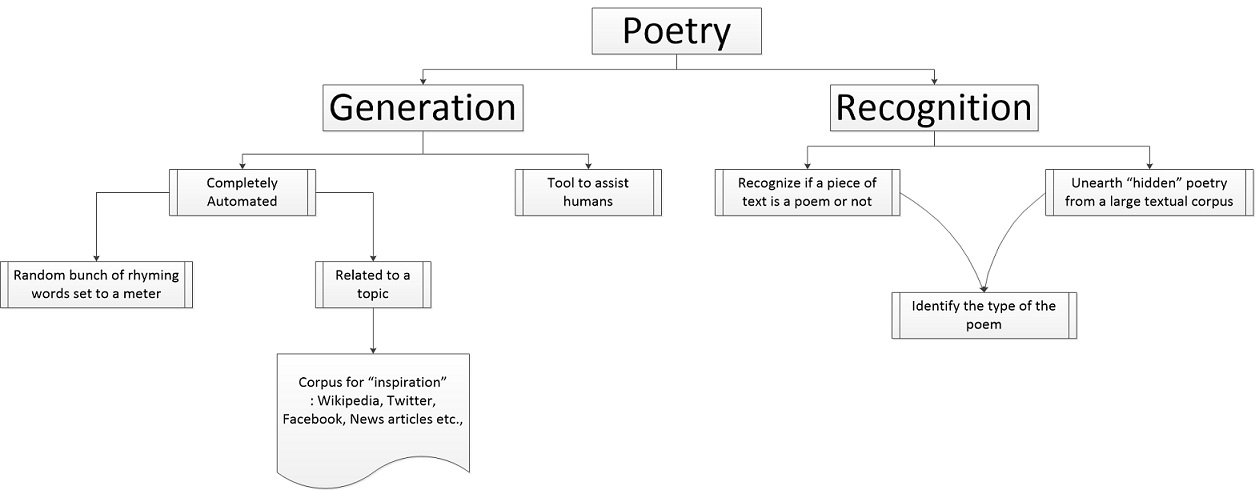
\includegraphics[scale=0.5]{Images/Big_Picture}
    \caption{Overall Scope of the Project}
  \label{big_picture}
\end{figure*}
\section{Data Structures}
\section{Algorithms}
\section{Interface Diagram}

\subsection{Poetry Recognizer}

\section{Data Structures}
\section{Algorithms}
\section{Interface Diagram}

\bibliographystyle{unsrt}
\bibliography{myrefs}
\end{document}
\end{document}